\documentclass[../../main/main.tex]{subfiles}
\graphicspath{{./figures/}}

\dominitoc
\faketableofcontents

% \renewcommand{\mtcSfont}{\small\bfseries}
% \renewcommand{\mtcSSfont}{\footnotesize}
\mtcsettitle{minitoc}{}
\mtcsetrules{*}{off}

\makeatletter
\renewcommand{\@chapapp}{\'Electrocin\'etique -- chapitre}
\renewcommand{\chaplett}{E}
\makeatother

% \toggletrue{student}
% \toggletrue{corrige}
% \renewcommand{\mycol}{black}
% \renewcommand{\mycol}{gray}

\hfuzz=5.003pt

\begin{document}
\setcounter{chapter}{1}

\settype{book}
\settype{prof}
\settype{stud}

\chapter{Dipôles et associations}

\vspace*{\fill}

\begin{tcn}(appl)<ctc>"somm"'t'{Sommaire}
	\let\item\olditem
	\vspace{-15pt}
	\minitoc
	\vspace{-25pt}
\end{tcn}

\begin{tcn}[sidebyside](appl)<ctb>"how"'t'{Capacités exigibles}
	\begin{itemize}[label=\rcheck]
		\item Connaître les relations entre l'intensité et la tension.
		\item Citer des ordres de grandeurs des composants R, L, C.
		\item Exprimer la puissance dissipée par effet \textsc{Joule} dans une
		      résistance.
		\item Exprimer l'énergie stockée dans un condensateur ou une bobine.
		\item Remplacer une association série ou parallèle de deux
		      résistances par une résistance équivalente.
		\item Établir et exploiter les relations des diviseurs de
		      tension ou de courant.
	\end{itemize}
	\tcblower
	\begin{itemize}[label=\rcheck]
		\item Modéliser une source en utilisant la représentation de
		      \textsc{Thévenin}.
		\item Évaluer une résistance d'entrée ou de sortie à
		      l'aide d'une notice ou d'un appareil afin d'appréhender les
		      conséquences de leurs valeurs sur le fonctionnement d'un circuit.
		\item Étudier l'influence des résistances d'entrée ou de
		      sortie sur le signal délivré par un GBF, sur la mesure effectuée par
		      un oscilloscope ou un multimètre.
	\end{itemize}
\end{tcn}

\vspace*{\fill}
\newpage
\vspace*{\fill}

%\vspace{-15pt}
\begin{tcn}[%
		sidebyside, fontupper=\small, fontlower=\small
	](appl)<ctb>"chek"'t'{L'essentiel}
	\begin{tcn}[nsp](defi)<ctc>'t'{Définitions}
		\tcblistof[\paragraph*]{defi}{\hspace*{4.8pt}}
	\end{tcn}
	% \begin{tcn}[nsp](rapp)<ctc>'t'{Rappels}
	% 	\tcblistof[\paragraph*]{rapp}{\hspace*{4.8pt}}
	% \end{tcn}
	\begin{tcn}[nsp](prop)<ctc>'t'{Propriétés}
		\tcblistof[\paragraph*]{prop}{\hspace*{4.8pt}}
		% \tcblistof[\paragraph*]{loi}{\hspace*{4.8pt}}
		% \tcblistof[\paragraph*]{theo}{\hspace*{4.8pt}}
	\end{tcn}
	% \begin{tcn}[nsp](loi)<ctc>'t'{Lois}
	% 	\tcblistof[\paragraph*]{loi}{\hspace*{4.8pt}}
	% \end{tcn}
	% \begin{tcn}[nsp](coro)<ctc>'t'{Corollaires}
	%   \tcblistof[\paragraph*]{coro}{\hspace*{4.8pt}}
	% \end{tcn}
	% \begin{tcn}[nsp](demo)<ctc>'t'{Démonstrations}
	% 	\tcblistof[\paragraph*]{demo}{\hspace*{4.8pt}}
	% 	\tcblistof[\paragraph*]{prev}{\hspace*{4.8pt}}
	% \end{tcn}
	% \begin{tcn}[nsp](inte)<ctc>'t'{Interprétations}
	% 	\tcblistof[\paragraph*]{inte}{\hspace*{4.8pt}}
	% \end{tcn}
	% \begin{tcn}[nsp](impl)<ctc>'t'{Implications}
	% 	\tcblistof[\paragraph*]{impl}{\hspace*{4.8pt}}
	% \end{tcn}
	% \begin{tcn}[nsp](tool)<ctc>'t'{Outils}
	% 	\tcblistof[\paragraph*]{tool}{\hspace*{4.8pt}}
	% \end{tcn}
	% \begin{tcn}[nsp](nota)<ctc>'t'{Notations}
	% 	\tcblistof[\paragraph*]{nota}{\hspace*{4.8pt}}
	% \end{tcn}
	% \begin{tcn}[nsp](appl)<ctc>'t'{Applications}
	% 	\tcblistof[\paragraph*]{appl}{\hspace*{4.8pt}}
	% \end{tcn}
	% \begin{tcn}[nsp](rema)<ctc>'t'{Remarques}
	%   \tcblistof[\paragraph*]{rema}{\hspace*{4.8pt}}
	% \end{tcn}
	% \begin{tcn}[nsp](exem)<ctc>'t'{Exemples}
	%   \tcblistof[\paragraph*]{exem}{\hspace*{4.8pt}}
	% \end{tcn}
	% \begin{tcn}[nsp]*(ror)<ctc>"hart"'t'{Points importants}
	%   \tcblistof[\paragraph*]{ror}{\hspace*{4.8pt}}
	% \end{tcn}
	% \begin{tcn}[nsp](impo)<ctc>'t'{Erreurs communes}
	%   \tcblistof[\paragraph*]{impo}{\hspace*{4.8pt}}
	% \end{tcn}
	\tcblower
	% \begin{tcn}[nsp](defi)<ctc>'t'{Définitions}
	%   \tcblistof[\paragraph*]{defi}{\hspace*{4.8pt}}
	% \end{tcn}
	% \begin{tcn}[nsp](rapp)<ctc>'t'{Rappels}
	%   \tcblistof[\paragraph*]{rapp}{\hspace*{4.8pt}}
	% \end{tcn}
	% \begin{tcn}[nsp](prop)<ctc>'t'{Propriétés}
	% \tcblistof[\paragraph*]{prop}{\hspace*{4.8pt}}
	% \tcblistof[\paragraph*]{loi}{\hspace*{4.8pt}}
	% \tcblistof[\paragraph*]{theo}{\hspace*{4.8pt}}
	% \end{tcn}
	% \begin{tcn}[nsp](coro)<ctc>'t'{Corollaires}
	%   \tcblistof[\paragraph*]{coro}{\hspace*{4.8pt}}
	% \end{tcn}
	\begin{tcn}[nsp](demo)<ctc>'t'{Démonstrations}
		\tcblistof[\paragraph*]{demo}{\hspace*{4.8pt}}
		% \tcblistof[\paragraph*]{prev}{\hspace*{4.8pt}}
	\end{tcn}
	% \begin{tcn}[nsp](inte)<ctc>'t'{Interprétations}
	% 	\tcblistof[\paragraph*]{inte}{\hspace*{4.8pt}}
	% \end{tcn}
	\begin{tcn}[nsp](impl)<ctc>'t'{Implications}
		\tcblistof[\paragraph*]{impl}{\hspace*{4.8pt}}
	\end{tcn}
	% \begin{tcn}[nsp](tool)<ctc>'t'{Outils}
	%   \tcblistof[\paragraph*]{tool}{\hspace*{4.8pt}}
	% \end{tcn}
	% \begin{tcn}[nsp](nota)<ctc>'t'{Notations}
	% 	\tcblistof[\paragraph*]{nota}{\hspace*{4.8pt}}
	% \end{tcn}
	% \begin{tcn}[nsp](odgr)<ctc>'t'{Ordres de grandeur}
	% 	\tcblistof[\paragraph*]{odgr}{\hspace*{4.8pt}}
	% \end{tcn}
	\begin{tcn}[nsp](appl)<ctc>'t'{Applications}
		\tcblistof[\paragraph*]{appl}{\hspace*{4.8pt}}
	\end{tcn}
	% \begin{tcn}[nsp](rema)<ctc>'t'{Remarques}
	%   \tcblistof[\paragraph*]{rema}{\hspace*{4.8pt}}
	% \end{tcn}
	% \begin{tcn}[nsp](exem)<ctc>'t'{Exemples}
	% 	\tcblistof[\paragraph*]{exem}{\hspace*{4.8pt}}
	% \end{tcn}
	% \begin{tcn}[nsp](ror)<ctc>"hart"'t'{Points importants}
	% 	\tcblistof[\paragraph*]{ror}{\hspace*{4.8pt}}
	% \end{tcn}
	\begin{tcn}[nsp](impo)<ctc>'t'{Erreurs communes}
		\tcblistof[\paragraph*]{impo}{\hspace*{4.8pt}}
	\end{tcn}
\end{tcn}

\vspace*{\fill}

\newpage

\section{Généralité sur les dipôles}
\subsection{Caractéristique d'un dipôle}
\begin{tcbraster}[raster columns=2, raster equal height=rows]
	\begin{tcb*}[label=def:dipcara](defi){Caractéristique}

		On appelle \textbf{caractéristique} d'un dipôle la fonction $I = f(U)$
		(ou $U = g(I)$ selon la convention). Sauf indication contraire, elle est
		déterminée \textbf{en régime continu}.

		\tcbsubtitle{\fatbox{Cas particuliers}}
		\begin{itemize}
			\item \psw{%
				      \textbf{Court-circuit} (fil branché aux bornes) $\Ra $
				      $U = 0$, et ce pour tout $I$.
			      }%
			\item \psw{%
				      Un dipôle qui n'est
				      \textbf{pas relié à un circuit fermé} a pour intensité $I = 0$.
			      }%
		\end{itemize}
	\end{tcb*}
	\begin{tcb}[label=exem:dipcara](exem)<rgtt>'r'{}
		\begin{center}
			\sswitch{%
				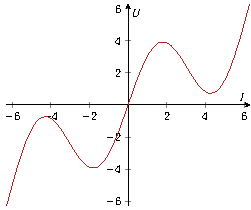
\includegraphics[width=.8\linewidth, draft=true]{carac_gen}
			}{%
				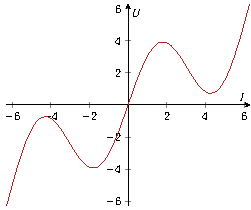
\includegraphics[width=.8\linewidth]{carac_gen}
			}%
			\captionof{figure}{}
		\end{center}
	\end{tcb}
\end{tcbraster}

\vspace{-10pt}
\subsection{Classification de dipôles}
\begin{tcb*}[label=def:actifpassif, fontupper=\small, tabularx={Y|Y|Y}]
	(defi){Vocabulaire des caractéristiques}
	\vspace{10pt}
	\tcbsubtitle{\fatbox{Passif}}
	\begin{itemize}
		\item \psw{%
			      \textbf{Pas} alimenté, récepteur.
		      }%
		\item \psw{%
			      \textbf{Passe par (0,0)}.
		      }%
	\end{itemize}
	&
	\vspace{-10pt}
	\tcbsubtitle{\fatbox{Linéaire}}
	\psw{%
		Un dipôle est dit \textbf{linéaire} si sa caractéristique est une
		\textbf{droite}.
	}%
	&
	\vspace{-10pt}
	\tcbsubtitle{\fatbox{Symétrique}}
	\psw{%
		\textbf{Symétrique} $\Lra$ \textbf{impaire}. \fbox{Symétrique $\Ra$ passif}.
	}%
	\\
	\vspace{-10pt}
	\tcbsubtitle{\fatbox{Actif}}
	\begin{itemize}
		\item \psw{%
			      \textbf{Est} alimenté, générateur.
		      }%
		\item \psw{%
			      \textbf{Passe pas par (0,0)}.
		      }%
	\end{itemize}
	&
	\vspace{-10pt}
	\tcbsubtitle{\fatbox{Non-linéaire}}
	\psw{%
		\textbf{Non-linéaire} si sa caractéristique n'est
		\textbf{pas une droite}.
	}%
	&
	\vspace{-10pt}
	\tcbsubtitle{\fatbox{Asymétrique}}
	\psw{%
		\textbf{Asymétrique} si sa caractéristique n'est \textbf{pas impaire}.
	}%
\end{tcb*}

\section{Résistance}
\subsection{Définition et schéma}

% Lorsqu'un courant circule dans un matériau conducteur, les électrons sont
% freinés par les atomes de celui-ci. Cet effet est maximal dans certains dipôles
% que l'on appellera des conducteurs ohmiques ou résistors. Par abus de langage,
% on désignera le composant par le même nom que la grandeur physique qui le
% caractérise~: la résistance.

\begin{tcb*}[label=def:resistance, sidebyside](defi){Résistor}
	Un résistor est un dipôle \textbf{récepteur}, dont la caractéristique en
	convention récepteur suit la \textbf{loi d'Ohm}~:
	\psw{%
		\[
			\boxed{U=RI}
			\Lra
			\boxed{GU=I}
		\]
	}%
	\vspace{-15pt}
	\tcblower
	\tcbsubtitle{\fatbox{Unités}}
	\begin{itemize}
		\item \psw{%
			      Résistance en Ohm ($\Omega$) avec $R > 0$.
		      }%
		\item \psw{%
			      Conductance \fbox{$G=1/R$} en Siemens (S).
		      }%
	\end{itemize}
\end{tcb*}

\begin{tcb*}[cnt, bld](impo)"bomb"{Relation courant-tension}
	En convention \textbf{générateur}, il faut donc prendre \textbf{l'opposé} de
	la relation~!
\end{tcb*}

\begin{tcbraster}[raster columns=2, raster equal height=rows]
	\begin{tcb*}[label=impl:resistance](impl){Puissance de $R$}
		En utilisant la caractéristique de la résistance et l'expression de la
		puissance d'un dipôle, on a
		\psw{%
			\[
				\boxed{P_{\text{reçue}} = RI^2 = \frac{U^2}{R} = GU^2}
			\]
		}%
		qui est positive. Dans le cas de la résistance, cette puissance est
		entièrement \textbf{dissipée} par effet \textsc{Joule}.
		% \tcblower
		% \begin{center}
		% 	\sswitch{%
		% 		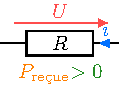
\includegraphics[width=.4\linewidth, draft=true]{resistance}
		% 	}{%
		% 		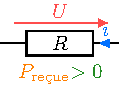
\includegraphics[width=.4\linewidth]{resistance}
		% 	}%
		% \end{center}
	\end{tcb*}
	\begin{tcb}[label=exem:resistance](exem)<rgtt>'r'{Caractéristique de $R$}
		\begin{center}
			\sswitch{%
				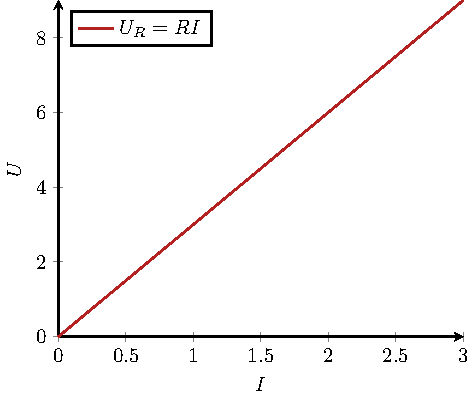
\includegraphics[width=.7\linewidth, draft=true]{carac_R}
			}{%
				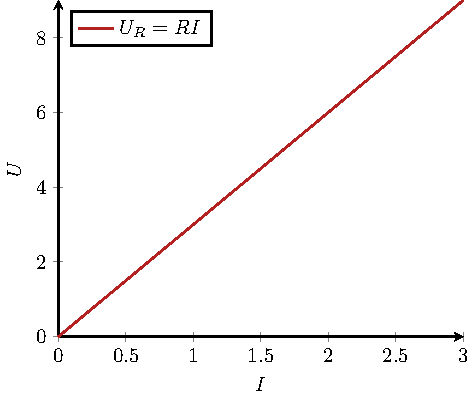
\includegraphics[width=.7\linewidth]{carac_R}
			}%
			\captionof{figure}{Caractéristique d'une résistance.}
		\end{center}
	\end{tcb}
\end{tcbraster}

\vspace{-15pt}
\subsection{Interrupteurs ouverts et fermés}
La valeur de la résistance permet de quantifier à quel poin le courant
circule ou non. Il y a alors deux situations extrêmes, celle pour $R = 0$ et
celle pour $R = +\infty$, qui correspondent à deux dipôles.

% \begin{tcb*}[sidebyside](defi){Interrupteurs ouvert et fermé}
% 	\tcbsubtitle{\fatbox{\textbf{Interrupteur ouvert}}}
% 	\psw{%
% 		\[
% 			\boxed{R = +\infty}
% 		\]
% 	}%
% 	\vspace{-15pt}
% 	\tcblower
% 	\tcbsubtitle{\fatbox{\textbf{Interrupteur fermé}}}
% 	\psw{%
% 		\[
% 			\boxed{R = 0}
% 		\]
% 	}%
% 	\vspace{-15pt}
% \end{tcb*}

\begin{tcb*}[sidebyside](prop){Interrupteurs ouvert et fermé}
	\tcbsubtitle{\fatbox{\textbf{Interrupteur ouvert}}}
	\begin{itemize}
		\item \psw{%
			      $R = +\infty$
		      }%
		\item \psw{%
			      $i = 0$~: un interrupteur ouvert \textbf{ne laisse pas passer le courant}.
		      }%
		\item \psw{%
			      $U \neq 0$~: il y a accumulation de charges d'un côté, donc une
			      \textbf{tension non nulle}.
		      }%
	\end{itemize}
	\vspace{-10pt}
	\noindent
	\hdashrule[0.5ex]{1\linewidth}{.5pt}{1mm}
	\sswitch{%
		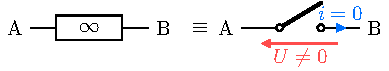
\includegraphics[width=\linewidth, draft=true]{inter_open}
	}{%
		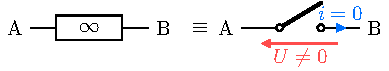
\includegraphics[width=\linewidth]{inter_open}
	}%
	\captionof{figure}{}
	\tcblower
	\tcbsubtitle{\fatbox{\textbf{Interrupteur fermé}}}
	\begin{itemize}
		\item \psw{%
			      $R = 0$
		      }%
		\item \psw{%
			      $i \neq 0$~: un interrupteur fermé \textbf{laisse passer le courant}.
		      }%
		\item \psw{%
			      $U = 0$~: il n'y a pas de différence de potentiel, donc la
			      \textbf{tension est nulle}.
		      }%
	\end{itemize}
	\vspace{-10pt}
	\noindent
	\hdashrule[0.5ex]{1\linewidth}{.5pt}{1mm}
	\sswitch{%
		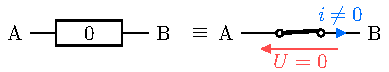
\includegraphics[width=\linewidth, draft=true]{inter_close}
	}{%
		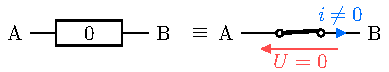
\includegraphics[width=\linewidth]{inter_close}
	}%
	\captionof{figure}{}
\end{tcb*}

\vspace{-10pt}
\subsection{Associations de résistances}
\subsubsection{Association de résistances en série}
\begin{tcb*}[label=prop:rserie, sidebyside, righthand ratio=.4](prop){Association en série}
	Des résistances $R_k$ en série forment un dipôle équivalent de
	résistance
	\psw{%
		\[
			% \boxed{R_{\equ} = R_1 + R_2}
			%    \qqou
			\boxed{R\ind{eq} = \sum_k R_k}
		\]
	}%
	On dit qu'\textbf{en série, les résistances s'ajoutent}.
	\tcblower
	\begin{center}
		\sswitch{%
			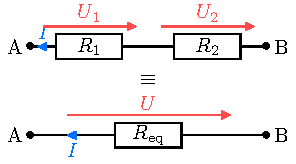
\includegraphics[width=\linewidth, draft=true]{rserie}
		}{%
			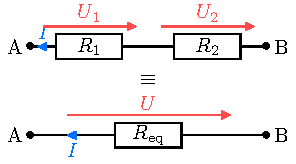
\includegraphics[width=\linewidth]{rserie}
			\captionof{figure}{}
		}%
	\end{center}
\end{tcb*}
\begin{tcb*}[label=demo:rserie, sidebyside, righthand ratio=.4](demo){Association en série}
	À partir du schéma précédent, on écrit la loi d'additivité des tensions,
	puis on applique la loi d'\textsc{Ohm} et on factorise.
	\smallbreak
	La démonstration s'étend naturellement avec la somme.
	\tcblower
	\psw{%
		\begin{align*}
			U         & = U_1 + U_2
			\\\Lra
			U         & = R_1I + R_2I
			\\\Lra
			U         & = (R_1 + R_2)I
			\\\Lra
			\Aboxed{U & = R\ind{eq}I}
			\qed
		\end{align*}
	}%
\end{tcb*}

\subsubsection{Association de résistances en parallèle}
\begin{tcb*}[label=prop:rpara, sidebyside, righthand ratio=.40](prop){Association en parallèle}
	Des résistances $R_k$ en dérivation forment un dipôle équivalent de résistance
	\psw{%
		\[
			\boxed{\frac{1}{R\ind{eq}} = \sum_k \frac{1}{R_k}}
			\Lra
			\boxed{G_{\equ} = \sum_k G_k}
		\]
	}%
	On dit qu'\textbf{en parallèle, l'inverse des résistances s'ajoutent}.
	\tcblower
	\begin{center}
		\sswitch{%
			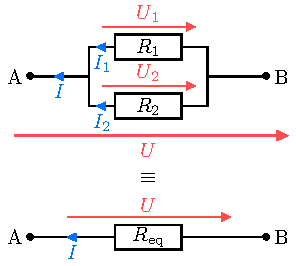
\includegraphics[width=\linewidth, draft=true]{rpara}
		}{%
			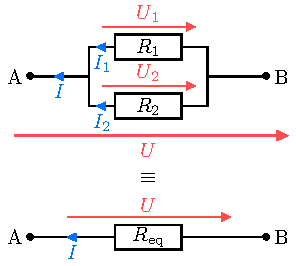
\includegraphics[width=\linewidth]{rpara}
		}%
		\captionof{figure}{}
	\end{center}
\end{tcb*}
\begin{tcb*}[label=demo:rpara, sidebyside](demo){Association en parallèle}
	\psw{%
		On applique la loi des nœuds et la loi d'\textsc{Ohm}~:
		\[
			I =
			I_1 + I_2 =
			\frac{U}{R_1} + \frac{U}{R_2} =
			\left(\dfrac{1}{R_1} + \dfrac{1}{R_2}\right) U
		\]
	}%
	\tcblower
	\psw{%
		Or, $I = \frac{U}{R\ind{eq}} = G\ind{eq}U$. Ainsi,
		On a bien l'expression d'un unique conducteur ohmique de résistance
		\[
			\boxed{\dfrac{1}{R_{\equ}} = \dfrac{1}{R_1} + \dfrac{1}{R_2}}
			\Lra
			\boxed{R_{\equ} = \frac{R_1R_2}{R_1 + R_2}}
			\qed
		\]
	}%
\end{tcb*}
\begin{tcb*}[breakable](appl)<lftt>{Résistance équivalente}
	\begin{isd}
		\vspace{-15pt}
		Exprimer en fonction de $R$ la résistance équivalente entre A et B pour
		l'association ci-dessous.
		\begin{center}
			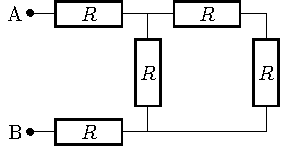
\includegraphics[width=.7\linewidth]{exer_rasso-plain}
		\end{center}
		\tcblower
		\vspace{-15pt}
		\psw{%
			\begin{align*}
				R_{\equ} & =
				\textcolor{\sswitch{white}{orange}}{R + R} +
				\textcolor{\sswitch{white}{brandeisblue}}{R\ind{eq,2}} \\ \Lra
				R_{\equ} & =
				\textcolor{\sswitch{white}{orange}}{2R} +
				\textcolor{\sswitch{white}{brandeisblue}}{%
					\frac{
						R\times \textcolor{\sswitch{white}{ForestGreen}}{R\ind{eq,1}}
					}{%
						R + \textcolor{\sswitch{white}{ForestGreen}}{R\ind{eq,1}}
					}%
				}%
				\\ \Lra
				R_{\equ} & =
				2R + \frac{
					R\times\textcolor{\sswitch{white}{ForestGreen}}{2R}
				}{%
					R+\textcolor{\sswitch{white}{ForestGreen}}{2R}
				}%
				\\ \Lra
				R_{\equ} & = 2R + \frac{2R^{\cancel{2}}}{3\cancel{R}}
				\\ \Lra
				R_{\equ} & = \frac{8R}{3}
			\end{align*}
		}%
		\vspace{-15pt}
	\end{isd}
	\vspace{-20pt}
	\tcblower
	\begin{center}
		\sswitch{%
			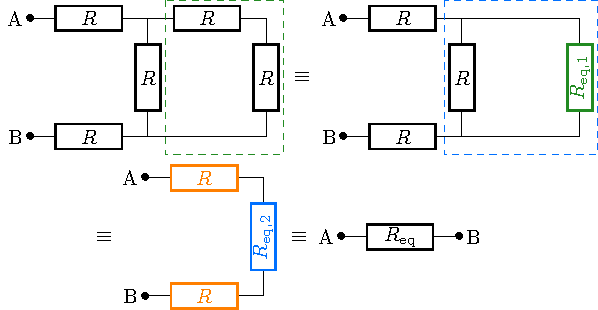
\includegraphics[width=\linewidth, draft=true]{exer_rasso}
		}{%
			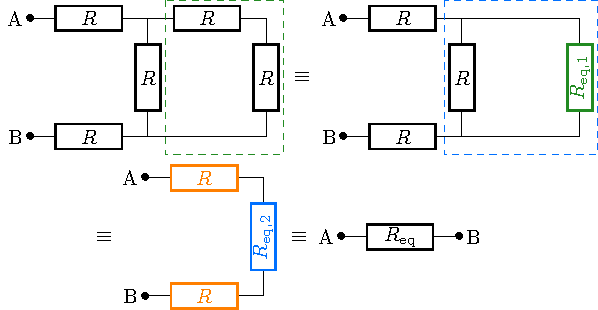
\includegraphics[width=\linewidth]{exer_rasso}
		}%
		\captionof{figure}{}
	\end{center}
	\vspace{-30pt}
\end{tcb*}

\subsection{Les ponts diviseurs}

% Les ponts diviseurs sont des relations permettant de trouver des courants ou des
% tensions dans certains cas particuliers, sans repasser par l'écriture des lois
% des nœuds, des mailles et d'\textsc{Ohm}.

% \vspace{-15pt}
\subsubsection{Pont diviseur de tension}

\begin{tcb*}[label=prop:divtens, sidebyside, righthand ratio=.4](prop){Pont
			diviseur de tension}
	Soit une branche de tension totale $U\ind{brch}$ connue, composée de
	résistances $R_k$. On cherche la tension $U_k$ d'une des résistances $R_k$ de
	la branche. Avec $R\ind{brch}$ la résistance équivalente de la branche, on a alors~:
	\psw{%
		\[
			\boxed{U_k = \frac{R_k}{R\ind{brch}}U\ind{brch}}
		\]
	}%
	\vspace{-15pt}
	\tcblower
	\begin{center}
		\sswitch{%
			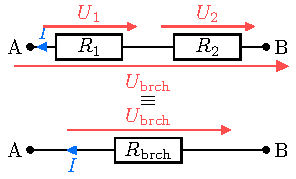
\includegraphics[width=\linewidth, draft=true]{rserie_divtens}
		}{%
			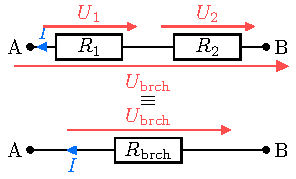
\includegraphics[width=\linewidth]{rserie_divtens}
		}%
		\captionof{figure}{}
	\end{center}
\end{tcb*}
\begin{tcb*}[label=demo:divtens](demo){Pont diviseur de tension}
	On part de ce qui est partagé dans le circuit, ici l'intensité~:
	\psw{%
		\begin{gather*}
			I = \frac{U\ind{brch}}{R\ind{brch}}
			\qet
			I = \frac{U_k}{R_k}
			\qqso
			\boxed{U_k = \frac{R_k}{R\ind{brch}U\ind{brch}}}
			\qed
		\end{gather*}
	}%
	\vspace{-15pt}
\end{tcb*}

\subsubsection{Pont diviseur de courant}

\begin{tcb*}[label=prop:divcour, sidebyside, righthand ratio=.4](prop){Pont diviseur de courant}
	Soit une maille parallèle d'intensité totale $I\ind{para}$ connue, de tension
	$U\ind{para}$. Les branches parallèles sont composées de
	résistances $R_k$. On cherche l'intensité $I_k$ d'une des résistances $R_k$ de
	la maille. Avec $R\ind{para}$ la résistance équivalente de la branche, on a alors~:
	\psw{%
		\[
			\boxed{I_k = \frac{R\ind{para}}{R_k}I\ind{para}}
			\Lra
			\boxed{I_k = \frac{G_k}{G\ind{para}}I\ind{para}}
		\]
	}%
	\vspace{-15pt}
	\tcblower
	\begin{center}
		\sswitch{%
			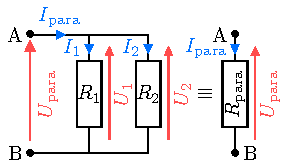
\includegraphics[width=\linewidth, draft=true]{divis_courant}
		}{%
			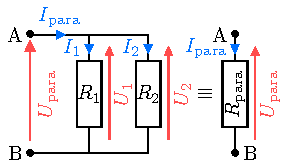
\includegraphics[width=\linewidth]{divis_courant}
		}%
		\captionof{figure}{}
	\end{center}
\end{tcb*}
\begin{tcb*}[label=demo:divcour](demo){Pont diviseur de courant}
	On part de ce qui est partagé dans le circuit, ici la tension~:
	\psw{%
		\begin{gather*}
			U\ind{parr} = R\ind{parr}I\ind{parr}
			\qet
			U\ind{parr} = R_kI_k
			\qqso
			\boxed{I_k = \frac{R\ind{parr}}{R_k}I\ind{parr}}
			\qed
		\end{gather*}
	}%
	\vspace{-15pt}
\end{tcb*}

% \vspace{-15pt}
\section{Sources}
\subsection{Sources de tension}

\begin{tcb*}[label=def:gentens, sidebyside, righthand ratio=.2](defi){Générateur
			idéal de tension}
	Il \textbf{impose une tension}, le courant débité est lui imposé par le reste
	du circuit électrique. Il est dit \textbf{idéal} si la tension imposée est
	\textbf{constante}, quel que soit le courant débité.
	\tcblower
	\vspace{-10pt}
	\begin{center}
		\sswitch{%
			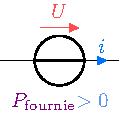
\includegraphics[width=.7\linewidth, draft=true]{gconvg}
		}{%
			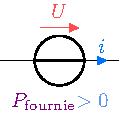
\includegraphics[width=.7\linewidth]{gconvg}
		}%
		\vspace{-10pt}
		\captionof{figure}{}
	\end{center}
\end{tcb*}

% \subsection{Source réelle de tension}
\begin{tcb*}[label=def:gentens, sidebyside, righthand ratio=.3](defi){Générateur
			réel de tension}
	À cause des effets résistifs, la tension imposée et le courant débité sont
	liés~:
	\psw{%
		\[\boxed{U = E_0 - ri}\]
	}%
	On parle de \textbf{générateur de Thévenin}, et $E_0$ est la \textbf{force
		électromotrice}.
	\tcblower
	\vspace{-10pt}
	\begin{center}
		\sswitch{%
			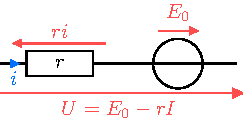
\includegraphics[width=.8\linewidth, draft=true]{thevenin}
		}{%
			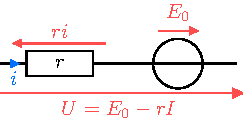
\includegraphics[width=.8\linewidth]{thevenin}
		}%
		\vspace{-10pt}
		\captionof{figure}{}
	\end{center}
\end{tcb*}

% \vspace{-10pt}
\begin{tcb*}[label=exem:gentens, sidebyside](exem)<lftt>{Caractéristique de
			générateurs de tension}
	\begin{center}
		\sswitch{%
			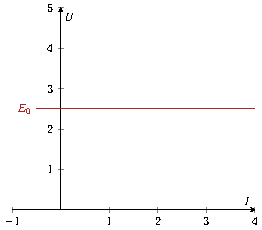
\includegraphics[width=.6\linewidth, draft=true]{carac_tens}
		}{%
			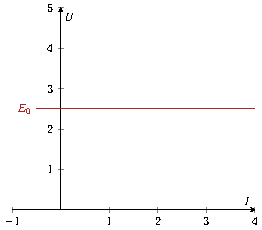
\includegraphics[width=.6\linewidth]{carac_tens}
		}%
		\captionof{figure}{Caractéristique idéale.}
		% \vspace{-15pt}
	\end{center}
	\tcblower
	\begin{center}
		\sswitch{%
			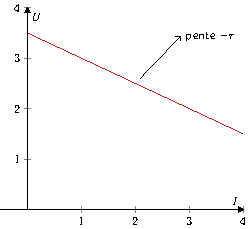
\includegraphics[width=.6\linewidth, draft=true]{carac_thev}
		}{%
			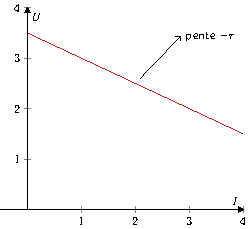
\includegraphics[width=.6\linewidth]{carac_thev}
		}%
		\captionof{figure}{Caractéristique réelle.}
		% \vspace{-15pt}
	\end{center}
\end{tcb*}

% \vspace{-15pt}
% \subsection{Résistance de sortie}

\begin{tcb*}[label=prop:rsortie, sidebyside, righthand ratio=.3](prop){Résistance de sortie}
	Un générateur réel de f.e.m. $E_0$ branché sur une résistance $R$ est un
	générateur idéal si la tension reçue par $R$ est très proche de $E_0$.
	Pour ce faire,
	\psw{%
		\[ \boxed{r \ll R}\]
	}%
	\tcblower
	\vspace{-10pt}
	\begin{center}
		\sswitch{%
			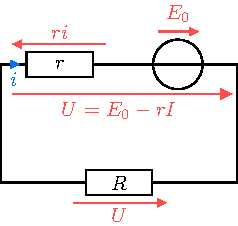
\includegraphics[width=.9\linewidth, draft=true]{rsortie}
		}{%
			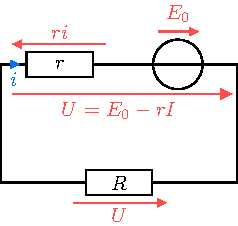
\includegraphics[width=.9\linewidth]{rsortie}
		}%
		\vspace{-10pt}
		\captionof{figure}{}
	\end{center}
\end{tcb*}
\begin{tcb*}[label=demo:rsortie](demo){Résistance de sortie}
	\psw{%
		On applique la formule du pont diviseur de tension pour avoir la tension
		$U$~:
		\[
			U = \frac{R}{R + r}E_0
		\]
		$U \neq E_0$ en général, mais si $R \gg r$ on a tout de même $U \approx
			E_0$.
		\hqed
	}%
\end{tcb*}

\subsection{Sources de courant}

\begin{tcb*}[label=def:gentens, sidebyside, righthand ratio=.2](defi){Générateur
			idéal de courant}
	Il \textbf{impose un courant}, la tension à ses bornes est lui imposé par le
	reste du circuit électrique. Il est dit \textbf{idéal} si le courant débité
	est constant quelle que soit la tension à ses bornes.
	\tcblower
	\vspace{-10pt}
	\begin{center}
		\sswitch{%
			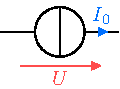
\includegraphics[width=.7\linewidth, draft=true]{gcourg}
		}{%
			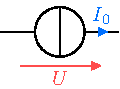
\includegraphics[width=.7\linewidth]{gcourg}
		}%
		\vspace{-10pt}
		\captionof{figure}{}
	\end{center}
\end{tcb*}

% \subsection{Complément~: source réelle de courant}
\begin{tcb*}[label=def:gencour, sidebyside, righthand ratio=.2](defi){Générateur réel de courant}
	À cause des effets résistifs, le courant imposé et la tension induite sont liés~:
	\psw{%
		\[
			\boxed{I = I_0 - \frac{U}{r_N}}
		\]
	}%
	On parle de \textbf{générateur de Norton}.
	\tcblower
	\vspace{-15pt}
	\begin{center}
		\sswitch{%
			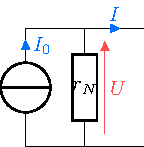
\includegraphics[width=.9\linewidth, draft=true]{norton}
		}{%
			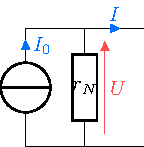
\includegraphics[width=.9\linewidth]{norton}
		}%
		\captionof{figure}{}
	\end{center}
\end{tcb*}

\begin{tcb*}[label=exem:gencour, sidebyside](exem)<lftt>{Caractéristique de
			générateurs de courant}
	\begin{center}
		\sswitch{%
			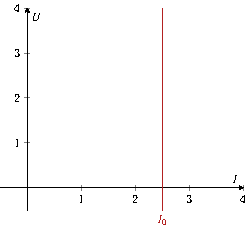
\includegraphics[width=.6\linewidth, draft=true]{carac_cour}
		}{%
			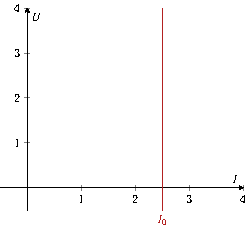
\includegraphics[width=.6\linewidth]{carac_cour}
		}%
		\captionof{figure}{Caractéristique idéale.}
		% \vspace{-15pt}
	\end{center}
	\tcblower
	\begin{center}
		\sswitch{%
			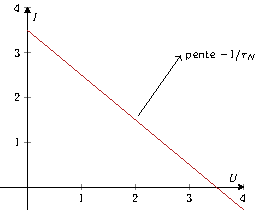
\includegraphics[width=.6\linewidth, draft=true]{carac_nort}
		}{%
			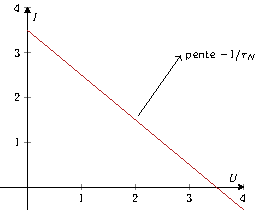
\includegraphics[width=.6\linewidth]{carac_nort}
		}%
		\captionof{figure}{Caractéristique réelle.}
		% \vspace{-15pt}
	\end{center}
\end{tcb*}

% \subsection{Résistance de sortie}

\begin{tcb*}[label=prop:rsortie, sidebyside, righthand ratio=.3](prop){Résistance de sortie}
	Un générateur réel de courant $I_0$ branché sur une résistance $R$ est un
	générateur idéal si le courant reçu par $R$ est très proche de $I_0$.
	Pour ce faire,
	\psw{%
		\[ \boxed{r_N \gg R}\]
	}%
	\tcblower
	\vspace{-15pt}
	\begin{center}
		\sswitch{%
			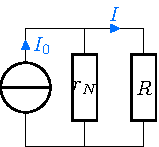
\includegraphics[width=.8\linewidth, draft=true]{rsortie_intens}
		}{%
			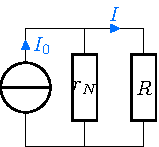
\includegraphics[width=.8\linewidth]{rsortie_intens}
		}%
		\captionof{figure}{}
	\end{center}
\end{tcb*}
\begin{tcb*}[label=demo:rsortie](demo){Résistance de sortie}
	\psw{%
		On applique la formule du pont diviseur de courant pour avoir le courant
		$I$~:
		\[ I = \frac{r_N}{r_N + R}I\]
		$I \neq I_0$ en général, mais si $R \ll r_N$ on a tout de même $I \approx
			I_0$.
		\hqed
	}%
\end{tcb*}

\subsection{Entraînements}
Donner les expressions de $U_1$, $U_2$, $U_3$ et $U_4$ en fonction de $E$
pour les schémas suivants.
\begin{tcb*}[tabularx={Y|Y|Y|Y}](appl)<lftt>{Pont diviseur de tension}
	\vspace{12pt}
	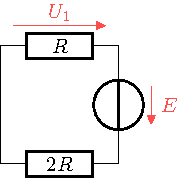
\includegraphics[scale=1]{pdt_a-plain}
	&
	\vspace{12pt}
	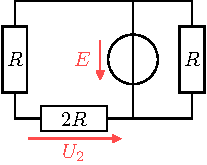
\includegraphics[scale=1]{pdt_b-plain}
	&
	\vspace{12pt}
	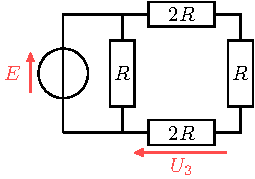
\includegraphics[scale=1]{pdt_c-plain}
	&
	\vspace{12pt}
	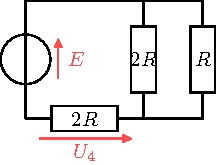
\includegraphics[scale=1]{pdt_d-plain}
	\\
	\begin{center}
		\sswitch{%
			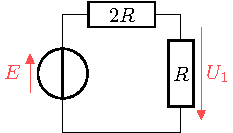
\includegraphics[width=\linewidth, draft=true]{pdt_a}
		}{%
			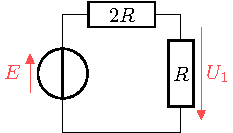
\includegraphics[width=\linewidth]{pdt_a}
		}%
	\end{center}
	\psw{%
		On a directement
		\[
			\boxed{U_1 = - \frac{1}{3}E}
		\]
	}%
	\vspace{-15pt}
	&
	\begin{center}
		\sswitch{%
			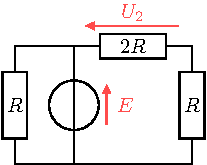
\includegraphics[width=\linewidth, draft=true]{pdt_b}
		}{%
			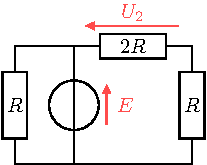
\includegraphics[width=\linewidth]{pdt_b}
		}%
	\end{center}
	\psw{%
		Avec la rotation du schéma, on voit facilement que
		\[
			\boxed{U_2 = \frac{2}{3}E}
		\]
	}%
	\vspace{-15pt}
	&
	\begin{center}
		\sswitch{%
			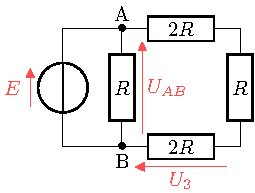
\includegraphics[width=\linewidth, draft=true]{pdt_c}
		}{%
			\includegraphics[width=\linewidth]{pdt_c}
		}%
	\end{center}
	\psw{%
		Ici, on remarque que $U_{AB} = E$. Ainsi
		\[
			\boxed{U_3 = - \frac{2}{5}E}
		\]
	}%
	\vspace{-15pt}
	&
	\begin{center}
		\sswitch{%
			\includegraphics[width=.8\linewidth, draft=true]{pdt_d}
		}{%
			\includegraphics[width=.8\linewidth]{pdt_d}
		}%
	\end{center}
	\psw{%
		$R\ind{eq,1} =\DS \frac{2R^{\cancel{2}}}{3\cancel{R}} = \frac{2R}{3}$,
		d'où
		\[
			\boxed{U_4 = \frac{3}{4}E}
		\]
	}%
	\vspace{-15pt}
\end{tcb*}

\begin{tcb*}[breakable, sidebyside, lefthand ratio=.3](appl)<lftt>{Pont diviseur de courant}
	Exprimer $I$ selon $I_0$.
	\begin{center}
		\includegraphics[scale=1]{divcour_last-plain}
	\end{center}
	\tcblower
	% \begin{center}
	% 	\sswitch{%
	% 		\includegraphics[width=\linewidth, draft=true]{divcour_last-a}
	% 	}{%
	% 		\includegraphics[width=\linewidth]{divcour_last-a}
	% 	}%
	% \end{center}
	\begin{isd}
		\psw{%
			\begin{gather*}
				\beforetext{On a}
				I = \frac{R\ind{para}}{r}I_0
				\\\beforetext{Or,}
				\frac{1}{R\ind{para}} = \frac{2}{r} + \frac{r}{2} = \frac{5}{2r}
			\end{gather*}
		}%
		\tcblower
		\psw{%
			\begin{gather*}
				\beforetext{Ainsi,}
				\boxed{I = \frac{2}{5}I_0}
			\end{gather*}
		}%
	\end{isd}
\end{tcb*}

\begin{tcb*}[label=impo:ponts](impo){Utilisation des ponts}
	\textbf{Attention} aux conditions d'application de ces formules~: résistances
	\textbf{en série} pour le pont diviseur de \textbf{tension}, et en
	\textbf{parallèle} pour le pont diviseur de \textbf{courant}.
	\smallbreak
	Si non, simplifier le circuit pour se ramener à cette forme. Vérifier
	également \textbf{le sens d'orientation des tensions et intensités}.
\end{tcb*}

\section{Condensateur et bobine}
\subsection{Présentation du condensateur}
\subsubsection{Composition}

Après les résistances, les condensateurs sont les composants les plus répandus
en électronique. Le condensateur est un composant électronique couramment
utilisé dans les circuits les plus divers : microprocesseurs, mémoires, horloges
électroniques, émetteurs et récepteurs radio, amplificateurs, etc.

\begin{tcb*}[label=def:condens, sidebyside, righthand ratio=.3](defi){Condensateur}
	Un condensateur est un composant constitué de deux \textbf{surfaces
		conductrices} appelées \textit{armatures} et séparées par un
	\textbf{matériau isolant}. Son symbole est représenté ci-contre.
	\tcblower
	\begin{center}
		\sswitch{%
			\includegraphics[width=.8\linewidth, draft=true]{condens_plain}
		}{%
			\includegraphics[width=.8\linewidth]{condens_plain}
		}%
		\captionof{figure}{}
	\end{center}
\end{tcb*}

\subsubsection{Relations fondamentales}
Quand un courant traverse le condensateur, des charges s'accumulent sur
les plaques~: si l'une est chargée $q$, l'autre est chargée $-q$.
\begin{tcb*}[label=prop:Ccondens, sidebyside, righthand ratio=.3](prop){Charge et capacité}
	La \textbf{tension à ses bornes} est \textbf{proportionnelle à $q$}, et on
	appelle ce coefficient de proportionnalité sa \textbf{capacité} notée $C$.
	On a donc
	\smallbreak
	\begin{isd}[sidebyside align=top]
		\psw{%
			\[\boxed{q = Cu}\]
		}%
		\vspace{-15pt}
		\tcblower
		\vspace{-10pt}
		\[
			\text{Unité~:~}
			\psw{%
				\text{$C$ en Farad (F)}
			}%
		\]
	\end{isd}
	\tcblower
	\vspace{-10pt}
	\begin{center}
		\sswitch{%
			\includegraphics[width=.8\linewidth, draft=true]{condens_q}
		}{%
			\includegraphics[width=.8\linewidth]{condens_q}
		}%
		\captionof{figure}{}
		\vspace{-10pt}
	\end{center}
\end{tcb*}

\begin{tcb*}(odgr)<lftt>{Valeurs de capacités}
	Le Farad est une «~grande~» unité~: on trouvera des valeurs entre le \si{mF}
	(\SI{e-3}{F}) et le \si{pF} (\SI{e-12}{F})~:
	\begin{itemize}
		\item En électronique, on est entre le \si{nF} et le \si{\micro F}~;
		\item En électrotechnique, on est plutôt de l'ordre de \SI{10}{mF}~;
		\item Une capacité parasite est autour du \si{pF}.
	\end{itemize}
\end{tcb*}

Pour \textbf{caractériser} le fonctionnement d'une capacité, on s'intéresse au
\textbf{lien} entre son \textbf{courant} et sa \textbf{tension}, comme on le
fait pour une résistance ($U = RI$). On remarque que~:
\begin{itemize}
	\item si $i > 0$, \psw{%
		      des charges arrivent sur l'armature de gauche, la charge
		      augmente donc la tension aussi~;
	      }%
	\item si $i < 0$, \psw{%
		      des charges repartent, la charge diminue donc la tension
		      aussi~;
	      }%
	\item si $i = 0$, \psw{%
		      aucune charge ne bouge, la quantité de charge sur l'armature
		      de gauche ne varie pas, la tension est constante.
	      }%
\end{itemize}

% Cette relation entre le \textbf{signe de $i$} et la \textbf{variation de $u$}
% suggère que $i$ est relié à la dérivée de $u$. On a alors~:

\begin{tcb*}[label=prop:Ccarac](prop){Relation courant-tension de $C$}
	Pour un condensateur \textbf{en convention récepteur}, l'intensité que
	le traverse s'exprime par
	\psw{%
		\[\boxed{i = C \dv{u_C}{t}}\]
	}%
	\vspace{-15pt}
\end{tcb*}
\begin{tcb*}[label=demo:Ccarac](demo){Relation courant-tension de $C$}
	Par définition de $i$ et de la charge,
	\psw{%
		\begin{DispWithArrows*}
			i & = \dv{q}{t}
			\Arrow{$q=Cu_C$}
			\\\Lra
			i & = C \dv{u_C}{t}
			\qed
		\end{DispWithArrows*}
	}%
	\vspace{-15pt}
\end{tcb*}

\subsubsection{Conditions limites}

\begin{tcb*}(prop){Conditions limites pour $C$}
	\begin{enumerate}
		\item La \textbf{tension} aux bornes d'un \textbf{condensateur} est
		      \textbf{continue}~;
		\item En régime \textbf{permanent}, le condensateur \textbf{bloque le
			      courant}.
	\end{enumerate}
\end{tcb*}
\begin{tcb*}(demo){Conditions limites pour $C$}
	\begin{enumerate}
		\item \psw{%
			      Si $u_C$ présente une variation brusque, alors $\dv{u_C}{t}$
			      devrait être infini. Or, comme $i = C \dv{u_C}{t}$, ceci n'est pas
			      possible puisque ça impliquerait que le courant le soit.
		      }%
		\item \psw{%
			      En régime permanent (continu), les tensions et courants ne dépendent
			      pas du temps. Alors $i = C \dv{u_C}{t} = 0$~: c'est un
			      \textbf{interrupteur ouvert}.
		      }%
	\end{enumerate}
\end{tcb*}

% \begin{tcbraster}[raster columns=2, raster equal height=rows]
% 	\begin{tcb*}[label=impl:continuité](impl){Continuité}
% 		\begin{framed}
% 			\psw{%
% 				La tension $u_C(t)$ aux bornes d'un condensateur ne peut pas
% 				varier instantanément, c'est une fonction continue.
% 			}%
% 		\end{framed}
% 	\end{tcb*}
% 	\begin{tcb*}*[label=impl:permanent](impl)"limp"'r'{Régime continu}
% 		En régime permanent (continu), les tensions et courants ne dépendent pas
% 		du temps. Alors $i = C \dv{u_C}{t} = 0$, ainsi
% 		\begin{framed}
% 			\psw{%
% 				En régime permanent, le condensateur se comporte comme un
% 				interrupteur ouvert et bloque le courant.
% 			}%
% 		\end{framed}
% 	\end{tcb*}
% \end{tcbraster}

\subsubsection{Associations}
\begin{tcb*}[label=prop:cserie, sidebyside](prop){Association $C$ en série}
	Deux condensateurs $C_1$ et $C_2$ en série forment un dipôle équivalent de
	capacité
	\psw{%
		\[
			\boxed{\dfrac{1}{C\ind{eq}} = \dfrac{1}{C_1} + \dfrac{1}{C_2}}
		\]
	}%
	On dit qu'\textbf{en série, l'inverse des capacités s'ajoutent}.
	\tcblower
	\begin{center}
		\sswitch{%
			\includegraphics[width=.8\linewidth, draft=true]{cserie}
		}{%
			\includegraphics[width=.8\linewidth]{cserie}
		}%
		\captionof{figure}{}
	\end{center}
\end{tcb*}
\begin{tcb*}[label=demo:cserie](demo){Association $C$ en série}
	On part ici de l'additivité des tensions~:
	\psw{%
		\begin{DispWithArrows*}
			u & = u_1 + u_2
			\CArrow{$\dv{t}\/(\cdot)$}
			\\\Lra
			\dv{u}{t} & = \dv{u_1}{t} + \dv{u_2}{t}
			\Arrow{$\dv{u}{t} = \frac{i}{C\ind{eq}}$}
			\\\Lra
			\frac{i}{C\ind{eq}} & = \left(\frac{1}{C_1} + \frac{1}{C_2}\right)i
			\Arrow{$\forall i$}
			\\\Lra
			\Aboxed{\frac{1}{C\ind{eq}} & = \frac{1}{C_1} + \frac{1}{C_2}}
			\qed
		\end{DispWithArrows*}
	}%
	\vspace{-15pt}
\end{tcb*}

\begin{tcb*}[label=prop:cpara, sidebyside](prop){Association $C$ en parallèle}
	Deux condensateurs $C_1$ et $C_2$ en dérivation forment un dipôle
	équivalent de capacité
	\psw{%
		\[
			\boxed{C\ind{eq} = C_1 + C_2}
		\]
	}%
	On dit qu'\textbf{en parallèle, les capacités s'ajoutent}.
	\tcblower
	\begin{center}
		\sswitch{%
			\includegraphics[width=\linewidth, draft=true]{cpara}
		}{%
			\includegraphics[width=\linewidth]{cpara}
		}%
		\captionof{figure}{}
	\end{center}
\end{tcb*}
\begin{tcb*}[label=demo:cpara](demo){Association $C$ en parallèle}
	On part ici de l'additivité des courants~:
	\psw{%
		\begin{DispWithArrows*}[]
			i &= i_1 + i_2
			\Arrow{$i = C\ind{eq}\dv{u}{t}$}
			\\\Lra
			C\ind{eq} \dv{u}{t} &= C_1 \dv{u}{t} + C_2 \dv{u}{t}
			\Arrow{$\forall u$}
			\\\Lra
			\Aboxed{C\ind{eq} &= C_1 + C_2}
			\qed
		\end{DispWithArrows*}
	}%
	\vspace{-15pt}
\end{tcb*}

\vspace{-15pt}
\subsubsection{Condensateur réel}

\begin{tcb*}[sidebyside, righthand ratio=.3](defi){Condensateur réel}
	Dans la réalité, un condensateur possède des \textbf{effets résistifs}.
	Les deux armatures d'un condensateur réel sont séparés par un matériau qui
	conduit très légèrement le courant. Ainsi, un condensateur réel se
	modélise par un \textbf{condensateur idéal} en \textbf{parallèle avec une
		résistance} $R_f$, nommée résistance de fuite, avec
	\psw{%
		\[
			\xul{R_f \approx \SI{e7}{\ohm}}
		\]
	}%
	\vspace{-15pt}
	\tcblower
	\begin{center}
		\sswitch{%
			\includegraphics[width=\linewidth, draft=true]{creel}
		}{%
			\includegraphics[width=\linewidth]{creel}
		}%
		\vspace{-15pt}
		\captionof{figure}{}
		\label{fig:creel}
	\end{center}
\end{tcb*}

\vspace{-15pt}
\subsubsection{Énergie stockée dans un condensateur}

\begin{tcb*}[label=prop:Ec](prop){Énergie stockée dans $C$}
	\psw{%
	\[
		\boxed{\Ec_C(t) = \frac{1}{2}C u_C{}^2(t)}
	\]
	}%
	\vspace{-10pt}
\end{tcb*}

\begin{tcb*}(demo){Énergie stockée dans $C$}
	\textbf{En convention récepteur}, la puissance \textbf{reçue} est
	\psw{%
		\begin{DispWithArrows*}
			\Pc_{C} &= u_Ci
			\Arrow{$i = C \dv{u_C}{t}$}
			\\\Lra
			\Pc_{C} &= Cu_C \dv{u_C}{t} \triangleq \dv{\Ec_C}{t}
		\end{DispWithArrows*}
	}%
	\vspace{-15pt}
	\leftcenters{\hspace{-12pt}Or, $\forall f$ fonction dérivable,}
	{\psw{$\DS\boxed{f\times f' = \left( \frac{1}{2}f^2 \right)'}$}}
	\smallbreak
	\begin{gather*}
		\beforetext{Ainsi,}
		\psw{%
			\Pc_{C} = \dv{t} \left( \frac{1}{2} Cu_C{}^2 \right)
			\Rightarrow \Ec_C(t) = \frac{1}{2}C u_C(t)^2
			\qed
		}%
	\end{gather*}
	\vspace{-15pt}
\end{tcb*}

\begin{tcb}[label=rema:genrec, sidebyside](rema)<lftt>{Condensateur récepteur ou
			générateur}
	Par l'étude de la relation précédente,
	\psw{%
		\[
			u_C \nearrow \quad \Ra \dv{u_C}{t} > 0 \Rightarrow \Pc_{C} > 0
		\]
	}%
	ainsi, le condensateur reçoit bien de l'énergie au reste du circuit, et il se
	\textbf{comporte comme récepteur}.
	\tcblower
	À l'inverse, on lit que
	\psw{%
		\[
			u_C \searrow \quad \Ra \dv{u_C}{t} < 0 \Rightarrow \Pc_{C} < 0
		\]
	}%
	ainsi, le condensateur cède en réalité de l'énergie au reste du circuit,
	autrement dit \textbf{il peut se comporter comme générateur}~!
\end{tcb}

\subsection{Présentation de la bobine}
\subsubsection{Composition}

Les bobines sont fréquemment utilisées dans les applications électrotechniques
(moteurs électriques, transformateurs). Comme elles sont lourdes et
encombrantes, elles sont plus rares en électronique.

\begin{tcb*}[label=def:bobine, sidebyside, righthand ratio=.3](defi){Bobine}
	Une bobine est constituée de l'enroulement régulier d'une grande
	longueur d'un fil métallique, recouvert d'une gaine ou d'un vernis
	isolant. Son symbole est représenté ci-contre.
	\tcblower
	\begin{center}
		\sswitch{%
			\includegraphics[width=.8\linewidth, draft=true]{bobine_plain}
		}{%
			\includegraphics[width=.8\linewidth]{bobine_plain}
		}%
		\captionof{figure}{}
	\end{center}
\end{tcb*}

\vspace{-15pt}
\subsubsection{Relation courant-tension}

\begin{tcb*}[label=prop:Lcarac, sidebyside, righthand ratio=.3](prop){Relation
			courant-tension}
	Quand un courant traverse la bobine, une \textbf{tension apparaît} à ses
	bornes. \textbf{En convention récepteur}, celle-ci s'exprime, avec $L$
	l'\textbf{inductance}~:
	\smallbreak
	\begin{isd}[sidebyside align=top]
		\psw{%
			\[\boxed{u_L = L\dv{i}{t}}\]
		}%
		\vspace{-15pt}
		\tcblower
		\vspace{-10pt}
		\[
			\text{Unité~:~}
			\psw{%
				\text{$L$ en Henry (H)}
			}%
		\]
	\end{isd}
	\tcblower
	\vspace{-10pt}
	\begin{center}
		\sswitch{%
			\includegraphics[width=.8\linewidth, draft=true]{bobine_u}
		}{%
			\includegraphics[width=.8\linewidth]{bobine_u}
		}%
		\vspace{-10pt}
		\captionof{figure}{}
	\end{center}
\end{tcb*}

\begin{tcb*}(odgr)<lftt>{Valeurs d'inductances}
	Le Henry est également une grande unité~: on trouvera des valeurs
	entre le \si{H} et le \si{\micro H} (\SI{e-6}{H}).
\end{tcb*}

\vspace{-25pt}
\subsubsection{Conditions limites}

\begin{tcb*}(prop){Conditions limites pour $L$}
	\begin{enumerate}
		\item L'\textbf{intensité} traversant une \textbf{bobine} est
		      \textbf{continue}~;
		\item En régime \textbf{permanent}, la bobine \textbf{laisse passer le
			      courant}.
	\end{enumerate}
\end{tcb*}
\begin{tcb*}(demo){Conditions limites pour $L$}
	\begin{enumerate}
		\item \psw{%
			      Si $i$ présente une variation brusque, alors $ \dv{i}{t}$ devrait
			      être infini. Or, comme $u_L = L\dv{i}{t}$, ceci n'est pas possible
			      puisque ça impliquerait que la tension le soit.
		      }%
		\item \psw{%
			      En régime permanent (continu), les tensions et courants ne dépendent
			      pas du temps. Alors $u_L = L \dv{i}{t} = 0$~: c'est \textbf{un fil}.
		      }%
	\end{enumerate}
\end{tcb*}

\vspace{-15pt}
\subsubsection{Associations}
\begin{tcb*}[label=prop:bserie, sidebyside, righthand ratio=.4]
	(prop){Association $L$ en série}
	Deux bobines $L_1$ et $L_2$ en série forment un dipôle équivalent
	d'inductance
	\psw{%
		\[
			\boxed{L\ind{eq} = L_1 + L_2}
		\]
	}%
	On dit qu'\textbf{en série, les inductances s'ajoutent}.
	\tcblower
	\vspace{-10pt}
	\begin{center}
		\sswitch{%
			\includegraphics[width=.8\linewidth, draft=true]{bserie}
		}{%
			\includegraphics[width=.8\linewidth]{bserie}
		}%
		\vspace{-10pt}
		\captionof{figure}{}
	\end{center}
\end{tcb*}
\begin{tcb*}[label=demo:bserie](demo){Association $L$ en série}
	On part de l'additivité des tensions~:
	\psw{%
		\vspace{-15pt}
		\begin{DispWithArrows*}
			u & = u_1 + u_2
			\Arrow{$u_L = L \dv{i}{t}$}
			\\\Lra
			L\ind{eq} \dv{i}{t} & = L_{1} \dv{i}{t} + L_{2} \dv{i}{t}
			\Arrow{$\forall i$}
			\\\Lra
			\Aboxed{L\ind{eq} &= L_1 + L_2}
			\qed
		\end{DispWithArrows*}
	}%
\end{tcb*}

\begin{tcb*}[label=prop:bpara, sidebyside](prop){Association $L$ en parallèle}
	Deux bobines $L_1$ et $L_2$ en dérivation forment un dipôle
	équivalent d'inductance
	\psw{%
		\[
			\boxed{\dfrac{1}{L\ind{eq}} = \dfrac{1}{L_1} + \dfrac{1}{L_2}}
		\]
	}%
	On dit qu'\textbf{en parallèle, l'inverse des inductances s'ajoutent}.
	\tcblower
	\begin{center}
		\sswitch{%
			\includegraphics[width=\linewidth, draft=true]{bpara}
		}{%
			\includegraphics[width=\linewidth]{bpara}
		}%
		\captionof{figure}{}
	\end{center}
\end{tcb*}
\begin{tcb*}[label=demo:bpara](demo){Association $L$ en parallèle}
	On part de l'additivité des courants~:
	\psw{%
		\begin{DispWithArrows*}[]
			i &= i_1+i_2
			\Arrow{$\dv{t}(~)$}
			\\\Ra
			\dv{i}{t} &= \dv{i_1}{t} + \dv{i_2}{t}
			\Arrow{$u_L = L \dv{i}{t}$}
			\\\Lra
			\frac{u}{L\ind{eq}} &= \frac{u}{L_1} + \frac{u}{L_2}
			\Arrow{$\forall u$}
			\\\Lra
			\Aboxed{\frac{1}{L\ind{eq}} &= \frac{1}{L_1} + \frac{1}{L_2}}
			\qed
		\end{DispWithArrows*}
	}%
	\vspace{-15pt}
\end{tcb*}

\subsubsection{Bobine réelle}

\begin{tcb*}[sidebyside, righthand ratio=.3](defi){Bobine réelle}
	Dans la réalité, le fil de cuivre enroulé possède une \textbf{résistance non
		nulle}. Une bobine réelle se modélise donc par une \textbf{bobine idéale}
	\textbf{en série avec une résistance} électrique $r$, avec
	\psw{%
		\[
			\xul{r \approx \SI{10}{\ohm}}
		\]
	}%
	\vspace{-15pt}
	\tcblower
	\begin{center}
		\sswitch{%
			\includegraphics[width=\linewidth, draft=true]{breel}
		}{%
			\includegraphics[width=\linewidth]{breel}
		}%
		\vspace{-15pt}
		\captionof{figure}{}
		\label{fig:breel}
	\end{center}
\end{tcb*}

\subsubsection{Énergie stockée dans une bobine}
\begin{tcb*}[label=prop:El](prop){Énergie stockée dans une bobine}
	\psw{%
		\[
			\boxed{\Ec_L(t) = \frac{1}{2}L i{}^2(t)}
		\]
	}%
	\vspace{-10pt}
\end{tcb*}

\begin{tcb*}(demo){Énergie stockée dans une bobine}
	\textbf{En convention récepteur}, la puissance \textbf{reçue} est
	\psw{%
		\begin{DispWithArrows*}
			\Pc_{L} &= u_Li
			\Arrow{$u_L = L \dv{i}{t}$}
			\\\Lra
			\Pc_{L} &= Li \dv{i}{t} \triangleq \dv{\Ec_L}{t}
		\end{DispWithArrows*}
	}%
	\vspace{-15pt}
	\leftcenters{\hspace{-12pt}Or, $\forall f$ fonction dérivable,}
	{\psw{$\DS\boxed{f\times f' = \left( \frac{1}{2}f^2 \right)'}$}}
	\smallbreak
	\begin{gather*}
		\beforetext{Ainsi,}
		\psw{%
			\Pc_{L} = \dv{t} \left( \frac{1}{2} Li{}^2 \right)
			\Rightarrow \Ec_C(t) = \frac{1}{2}L i(t)^2
			\qed
		}%
	\end{gather*}
	\vspace{-15pt}
\end{tcb*}

\begin{tcb}[label=rema:genrec, sidebyside](rema)<lftt>{Bobine réceptrice ou
			génératrice}
	Par l'étude de la relation précédente,
	\psw{%
		\[
			i \nearrow \quad \Ra \dv{i}{t} > 0 \Rightarrow \Pc_{L} > 0
		\]
	}%
	ainsi, la bobine reçoit bien de l'énergie au reste du circuit, et elle se
	\textbf{comporte comme un récepteur}.
	\tcblower
	À l'inverse, on lit que
	\psw{%
		\[
			i \searrow \quad \Ra \dv{i}{t} < 0 \Rightarrow \Pc_{L} < 0
		\]
	}%
	ainsi, la bobine cède en réalité de l'énergie au reste du circuit,
	autrement dit \textbf{elle peut se comporter comme un générateur}~!
\end{tcb}

\end{document}
